% TEMPLATE for Usenix papers, specifically to meet requirements of
%  USENIX '05
% originally a template for producing IEEE-format articles using LaTeX.
%   written by Matthew Ward, CS Department, Worcester Polytechnic Institute.
% adapted by David Beazley for his excellent SWIG paper in Proceedings,
%   Tcl 96
% turned into a smartass generic template by De Clarke, with thanks to
%   both the above pioneers
% use at your own risk.  Complaints to /dev/null.
% make it two column with no page numbering, default is 10 point

% Munged by Fred Douglis <douglis@research.att.com> 10/97 to separate
% the .sty file from the LaTeX source template, so that people can
% more easily include the .sty file into an existing document.  Also
% changed to more closely follow the style guidelines as represented
% by the Word sample file. 

% Note that since 2010, USENIX does not require endnotes. If you want
% foot of page notes, don't include the endnotes package in the 
% usepackage command, below.

% This version uses the latex2e styles, not the very ancient 2.09 stuff.
\documentclass[letterpaper,twocolumn,10pt]{article}
\usepackage{usenix,epsfig,endnotes}

\usepackage{booktabs} % For formal tables
\usepackage{epigraph}
\usepackage{afterpage}
\usepackage{tikz}
\usepackage{soul}
\usepackage[framemethod=tikz]{mdframed}
\usetikzlibrary{arrows,chains,decorations.pathreplacing}
\usepackage{pifont} % http://ctan.org/pkg/pifont
\usepackage{amsmath}
\usepackage{amsfonts}
\usepackage{amsthm}

\newcommand{\beq}{\begin{eqnarray}}
\newcommand{\eeq}{\end{eqnarray}}
\newcommand{\bhlpar}{\begin{mdframed}[innerleftmargin=0,innerrightmargin=0,hidealllines=true,backgroundcolor=yellow!20]}
\newcommand{\ehlpar}{\end{mdframed}}
\DeclareMathOperator{\wbf}{wBF}
\newtheorem{theorem}{Theorem}
\newcommand{\cmark}{\ding{51}}
\newcommand{\xmark}{\ding{55}}

\begin{document}

%don't want date printed
\date{}

%make title bold and 14 pt font (Latex default is non-bold, 16 pt)
\title{\Large \bf Towards Attack-Tolerant Networks: Concurrent mutlipath routing and the butterfly network}

%for single author (just remove % characters)
\author{
{\rm Anonymous}\\
For Blind Review
%\author{
%{\rm Edward L.\ Platt}\\
%University of Michigan School of Information
%\and
%{\rm Daniel M.\ Romero}\\
%University of Michigan School of Information
% copy the following lines to add more authors
% \and
% {\rm Name}\\
%Name Institution
} % end author

\maketitle

% Use the following at camera-ready time to suppress page numbers.
% Comment it out when you first submit the paper for review.
\thispagestyle{empty}


\subsection*{Abstract}
It is crucial for large-scale communication networks such as the internet
to be resilient against attacks \cite{sterbenz_resilience_2010}
such as censorship and surveillance,
which pose a threat to free expression and free association.
Self-organized networks such as the internet’s router network typically have
heavy-tailed degree distributions \cite{barabasi_scale-free_2009},
making them highly vulnerable to targeted attacks against central nodes
\cite{albert_error_2000}.
While cryptographic solutions exist,
they fail to address the underlying topological problem,
and remain vulnerable to
man-in-the-middle attacks \cite{nayak_different_2010}
and coercion \cite{grewal_caveat_2013}.
Coercion-resistant, topological approaches to attack tolerance are needed to
address the current vulnerability of communications infrastructure to
censorship and surveillance.
We present a novel concurrent multipath routing (CMR) algorithm for the
wraparound butterfly network topology,
as well as a highly attack-tolerant Structured Multipath Fault Tolerance (SMFT)
architecture which incorporates the butterfly CMR algorithm.
Our work is the first theoretical demonstration of a point-to-point
communication network architecture that can resist coercion and other
non-technical attacks, without requiring transitive trust.
To address cases where the network structure cannot be fully controlled,
we demonstrate how a snapshot of the internet's router network can be partially
rewired for greater attack-tolerance.

\section{Introduction}

\epigraph{The Net interprets censorship as damage and routes around it.}{\textit{--John Gilmore} \cite{elmer-dewitt_first_1993}}

Is it possible for any large-scale communication network to resist targeted
attacks?
The internet was originally designed to withstand targeted (nuclear) attacks
\cite{baran_distributed_1964},
and the resilience of the internet has long been part of common wisdom
\cite{elmer-dewitt_first_1993}.
But 18 years after Albert et al.\ \cite{albert_error_2000}
showed the internet's router network
is vulnerable to targeted attacks,
the fundamental problem of attack-tolerant network topology
remains unsolved.
Attack-tolerant topologies are desirable
for any physical or virtual network where a compromised node puts
communication at risk.
For example, the network of verified keys in the public key infrastructure
underlying secure http \cite{ellison_ten_2000},
or the network of DNS nameservers.
The ongoing vulnerability of the internet is evidenced by a long history of 
censorship and surveillance incidents achieved by means of targeted attacks
\cite{dainotti_analysis_2011}.
In this paper, we present the first theoretical network topology
supporting attack-toloerant, point-to-point networked communication,
without relying on transitive trust
\cite{christianson_why_1997}.

Methods for tolerating various kind of faults within networks are an
important and ongoing area of research
\cite{zin_survey_2015,albert_error_2000,sterbenz_resilience_2010}.
{\em Adversarial faults},
those in which an adversary can target attacks strategically,
deserve special attention.
Such attacks are both extremely difficult to guard against and 
often have important social implications.
In particular, censorship and surveillance are often achieved
by targeting central network locations and either blocking or capturing
the information flowing through them.
While cryptograpy can provide some protection against surveillance, it is
vulnerable to {\em man-in-the-middle} attacks \cite{nayak_different_2010},
and cannot overcome censorship when communication is blocked.
In this paper, we instead consider a topological approach.
The Internet's decentralized design was motivated
by the need to withstand targeted attacks, such as nuclear strikes
\cite{baran_distributed_1964}.
But despite longstanding common wisdom \cite{elmer-dewitt_first_1993},
both theoretical results and recent events
have demonstrated that the internet is surprisingly vulnerable to attack.

Analysis of the internet's router network has shown that while it
is remarkably resilient against random faults,
it is highly susceptible to adversarial faults \cite{albert_error_2000}.
These results have been attributed to the heavy-tailed
degree distribution of the Internet's router network
\cite{barabasi_emergence_1999,barabasi_scale-free_2009}.
Random failures are highly likely to affect only low-degree nodes,
thus having little effect.
However, adversarial faults target the few high-degree nodes,
and therefore remove a large number of edges with each fault.
So while the {\em protocols} of the Internet are decentralized,
the {\em network structure} is somewhat centralized. 
In other words, the protocols of the Internet do not {\em require}
centralization, but centralization may still emerge from the sociotechnical
processes that create its network structure.

The internet's vulnerability to censorship and other targeted attacks
has been demonstrated by several recent events.
In 2008, YouTube suffered a worldwide outage for several hours
when a service provider in Pakistan advertised false routing information
\cite{hunter_pakistan_2008}.
The action (known as a {\em black hole attack}) was intended to censor YouTube
within Pakistan only, but resulted in a worldwide cascading failure
when a router misconfiguration allowed the false routing information to
propagate outside of Pakistan.
This incident exemplifies the type of attack requiring a topological approach.
First, the attack was {\em non-technological} (a government order),
allowing the attacker to bypass any cryptographic or technology-based defenses.
Second, the attack originated at a {\em single point of failure}
(a misconfigured router).
Third, the behavior of the compromised component (the router) cascaded
through a {\em network} (the network of internet routers) because the correct
behavior of other components depended on the correct behavior
of the single point of failure.
And while the action was not an intentional attack against the global internet,
the ability of an attacker to succeed without even trying only highlights
the internet's vulnerability to adversarial faults.

Similarly, in 2013,
the Texas-based email provider Lavabit was ordered to disclose
their private SSL keys to the FBI \cite{poulsen_edward_2013}.
Lavabit instead chose to cease operations
in order to protect their users from surveillance.
Once again, the attack was non-technical.
And again, the attack was on a single point of failure:
Lavabit's web server and that server's SSL keys.
In this case, the affected network was the
internet's public key infrastructure.
With the private keys, an attacker would be able to intercept and
surveil traffic because the users would incorrectly trust that they were
communicating with Lavabit.
So we see that such vulnerabilities are not limited to any one system,
but result from centralized structure itself.

This paper addresses the need for a theoretial understanding of network and
redundancy-based approaches to attack tolerance.
Our primary result is theoretical: an algorithm for constructing highly redundant
paths in a particular network topology,
suggesting the importance
of further theoretical and applied work.

We make two main contributions.
We prove that the number of 
$h$-internally vertex disjoint
paths between two nodes in
a wrap-around butterfly network
is at least $2^h$,
and present a scalable and efficient concurrent multipath routing (CMR) algorithm
to find these paths.
This result is combined with structured multipath fault-tolerance (SMFT)
to achieve a high level of attack-tolerance.
We also show that rewiring a the edges of the internet's router network to
resemble a butterfly network allows it to tolerate a higher number of failures
without fragmenting, and increases the effective redundancy in the presence
of a large number of adversarial faults.

\section{Background and Related Work}
\label{sec-related}

Centralized approaches to attack-tolerance
such as {\em public key infrastructure} (PKI)
suffer from a number of vulnerabilities
\cite{ellison_ten_2000}, including vulnerability to coercion,
which stems largely from the single points of failure inherent to
centralization.
The {\em web of trust} is a decentralized alternative
\cite{zimmermann_official_1995,richters_trust_2011}
but depends on the unrealistic assumption of trust transitivity
\cite{christianson_why_1997}.

Many distributed consensus protocols (e.g., cryptocurrencies)
are designed to tolerate arbitrary or adversarial faults.
Byzantine agreement protocols
\cite{lamport_byzantine_1982,castro_practical_1999}
provide tolerance against arbitrary faults (including attacks) under
some circumstances, but are limited to small networks due to poor scalability.
Proof-of-work \cite{dwork_pricing_1993,nakamoto_bitcoin:_2008} (blockchain)
systems provide better scalability,
but are wasteful of computational and energy resources,
and do not take advantage of trusted relationships.
Federated Byzantine Agreement (FBA) \cite{mazieres_stellar_2015}
is scalable, allows for flexible trust,
and is highly fault-tolerant on networks meeting specific requirements.
However, FBA does not provide a method for constructing networks to meet
those requirements.

All existing attack-tolerant networks we are aware of are content-addressable
networks (CANs) in which data is stored and retrieved based on key values,
rather than point-to-point networks, in which data is communicated between
two parties.
Fiat and Saia described a scheme that combines the butterfly topology
with expander graphs to create a highly censorship-resistant,
content-addressable network \cite{fiat_censorship_2002},
although this scheme requires high levels of data replication and indefinite
storage.
Perhaps the most mature structural solution is the Freenet collaboration
\cite{clarke_freenet:_2001}.
Freenet uses secret sharing
\cite{shamir_how_1979, blakley_safeguarding_1979}
and small-world routing
\cite{zhang_using_2002,kleinberg_small-world_2000}
to create a content-addressable network with a high level of both
confidentiality and censorship resistance.
Freenet guarantees that data is stored redundantly,
but still allows for centralized network structure,
and thus single points of failure,
as data travels from its origin to the redundant storage locations.
Unlike the above content-addressable networks, our architecture is purely network based
and does not require nodes to store data indefinitely.

{\em Multipath routing} protocols identify multiple paths between
source and destination
in contrast to traditional {\em unipath} routing, which uses
a single path.
The special case of {\em concurrent} multipath routing uses multiple paths
simultaneously.
Multipath routing has many applications, including reduced congestion,
increased throughput, and more reliability
\cite{qadir_exploiting_2015}.
Many of these routing protocols offer increased confidentiality
\cite{zin_survey_2015}.
Some approaches utilize redundant paths as backups for increased
fault tolerance
\cite{alrajeh_secure_2013},
and some specifically protect against adversarial faults
\cite{kohno_improvement_2012, khalil_unmask:_2010, lou_h-spread:_2006}.
Most work on multipath routing has been motivated by applications related to
wireless sensor networks (WSNs),
and have thus focused on ad-hoc, unstructured networks, often having a central
base station.
The method of Liu et al.
\cite{liu_secure_2012}
routes multiple messages first to random peers and then
to a central base station,
with the network edges constrained by sensors' physical location.
We have found very few examples of CMR applied to {\em adversarial}
fault tolerance in the existing literature,
and all have focused on ad-hoc wireless sensor networks, without attention
to the role of network structure.

Our proposed routing algorithm makes use of a
{\em structured network}, in which link structure is predetermined.
Structured networks have been a popular tool in parallel processing
architectures \cite{kshemkalyani_distributed_2008}.
More recently, peer-to-peer systems based on distributed hash tables have used
structured {\em overlay networks} to map table keys to local TCP/IP routes
\cite{lua_survey_2005,korzun_structured_2013}.
Such networks can be designed to have favorable structural and routing
properties,
which can be used to to improve attack-tolerance.

Our proposed architecture is differentiated from existing systems by several
properties.
Decentralized architectures are more resistant to coercion
\cite{grewal_caveat_2013}
and man-in-the-middle attacks \cite{nayak_different_2010}.
Topological approaches address the root cause of vulnerability
in heavy-tail networks,
rather than relying on technology that can be side-stepped through coercion.
The topological approach is also more sustainable than proof-of-work systems.
Point-to-point communication allows two individuals to exchange messages
without requiring large amounts of indefinite data storage on intermediate
nodes.

%\begin{table*}[t!]
%\caption{Comparison of attack-tolerant network communication architectures.\label{tab:compare}}
%\begin{center}
%\begin{tabular}{l|p{0.6in}p{0.6in}p{0.6in}p{0.6in}p{0.6in}}
%                              & Decentra-lized & Trust-based & Bounded-trust & Topo-logical & Point-to-point \\
%\hline
%PKI            &               & \cmark      & \cmark        &             & \cmark     \\
%Web of Trust   & \cmark        & \cmark      &               &             & \cmark     \\
%Freenet        & \cmark        & \cmark      & \cmark        &             &            \\
%FBA            & \cmark        & \cmark      & \cmark        &             & \cmark     \\
%Proof of Work  & \cmark        &             & \cmark        &             &            \\
%Fiat-Saia      & \cmark        & \cmark      & \cmark        & \cmark      &            \\
%SMFT           & \cmark        & \cmark      & \cmark        & \cmark      & \cmark     \\
%\hline
%\end{tabular}
%\end{center}
%\end{table*}

\section{Networks and Fault Tolerance}
\label{sec-ft}
\subsection{Multipath Fault Tolerance}

Standard fault tolerance methods
\cite{avizienis_basic_2004, von_neumann_probabilistic_1956}
use redundancy to detect and correct
statistically independent faults.
In complex networks however, faults can be correlated when,
for example, two messages pass through the same faulty node.
For now, let us assume our sender (Alice) and receiver (Bob) are connected
by $\delta$ {\em independent paths} such that no two paths contain the same
faulty node.
Let $k = \alpha\delta$ be the number of messages Alice can send and
$l = \beta\delta$ be the number of nodes Mal can compromise.
If Alice choses paths at random and Mal compromises paths at random,
the probability of blocking or altering all of Alice's messages can be
shown to be approximately:
\begin{eqnarray}
\label{eq:pf_approx}
p_f &\approx&
\frac{\sqrt{\beta(1-\alpha)}}{\sqrt{\beta-\alpha}}
\left[
    \left( \frac{\beta-\alpha}{1-\alpha} \right)^{\alpha}
    \left( \frac{\beta}{\beta-\alpha} \right)^{\beta}
    (1-\alpha)
\right]^{\delta}.
\end{eqnarray}

Fig. \ref{fig:pfail} shows the value of $p_f$
as a function of $k$ and $l$.
Eq. (\ref{eq:pf_approx}) shows that while $p_f$
depends on the fractions of
paths actually utilized $\alpha$ and compromised $\beta$,
it decreases exponentially with $\delta$.
This result is significant because
$\delta$ depends only on the network structure.
{\em Thus, the scheme can be effective, even when the number of paths used
$k$ is a small fraction of the channels available}.
In other words, this scheme exhibits a {\em stabilizing asymmetry:}
senders can tolerate attacks from significantly more powerful
adversaries.
Furthermore, this scheme requires only a small increase in network traffic
as long as the network provides a large number of independent paths $\delta$.

\begin{figure}[h]
\centerline{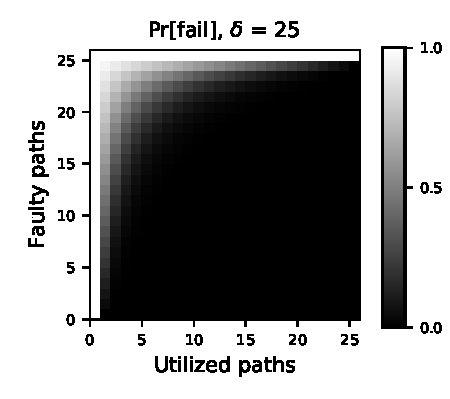
\includegraphics{fig-perror-25}}
\caption{
The probability of an undetectable error as a function of the number of
redundant channels and the number of adversarial faults.
A small increase in the number of utilized paths (network traffic)
can compensate for a large increase in attacker power.
}
\label{fig:pfail}
\end{figure}

\subsection{Effective Redundancy}

The effect of an attack on communication between two nodes
depends on how many of the paths between those nodes pass through
the a compromised node.
The number of such compromised paths depends on both the network topology
and the position of the endpoint nodes relative to the compromised node.
If the compromised node is one of the endpoints,
then all paths from that node are compromised.
When the endpoints are farther from the compromised node,
the paths from the endpoints branch out into many
paths before one of those passes through the compromised node.

The network topology determines how many redundant paths exist
less than a given distance $h$ away from each node.
With more paths, any single compromised node has a smaller effect.
For a given node pair $(s, t)$,
We call this number of paths $\delta_{h,s,t}$ the
{\em pairwise effective redundancy}.
For the entire network, the {\em effective redundancy} is the minimum over all
vertex pairs:
\beq
\delta_h(G) \equiv \min_{s,t \in V} \delta_{s,t,h}.
\eeq

In graph theoretical terms, the effective redundancy at distance $h$ is
the minimum number of $h${\em-internally vertex-disjoint} paths between any
node pair.
A higher effective redudncancy means that,
for a given distance $h$ between an endpoint and a compromised node,
the more redundant paths are available to route around that attack.
In the absence of centralized bottlenecks,
the effective redundancy is limited by the endpoint
closest to an attack.

\subsection{Structured Multipath Fault Tolerance}

Finding a maximal set of independent paths for an arbitrary network is NP hard
\cite{reiter_resilient_1998},
posing a challenge for multipath fault tolerance.
We propose side-stepping this problem by using structured networks,
for which independent paths can be generated efficiently.
We call this approach {\em structured multipath fault tolerance} (SMFT),
and now proceed to show how it is implemented on the butterfly
network topology.

\section{The Butterfly Network Topology}
\label{sec-butterfly}

In order to implement structured multipath fault tolerance,
we need a structured network topology with high effective redundancy.
In this paper, we apply SMFT to the butterfly network topology
\cite{kshemkalyani_distributed_2008}.
The butterfly network is recursive, with larger versions composed out of
multiple smaller versions,
suggesting large attack-tolerant networks could be constructed by merging smaller ones.
To address the case when the network cannot be fully controlled,
we show how partially rewiring a snapshot of the internet's router
network can greatly increase it's effective redundancy and
attack-tolerance properties, without requiring additional edges.

\subsection{Butterfly Network Topology}

We choose the butterfly topology
\cite{kshemkalyani_distributed_2008}
because of several desirable properties (described below)
and because its structure allows for relatively straightforward
design and analysis of routing algorithms.
While several variations on the butterfly network exist,
we utilize the $m$-dimensional, directed wrap-around butterfly,
denoted $\wbf(m)$:
\beq
\wbf(m) &=& (V, E_\downarrow \cup E_\rightarrow) \\
V &=& \mathbb{Z}_{m} \times \mathbb{Z}_2^m \\
E_\downarrow
&=&
\{((l,z),(l+1 \; (\text{mod } m),z) \} \\
E_\rightarrow
&=&
\{(l,z),(l+1 \; (\text{mod } m),
z \oplus 1_l \},
\eeq
where $\mathbb{Z}_m$ is the set of integers modulo $m$,
$\oplus$ represents component-wise addition modulo 2,
and $1_l$ is a vector with a 1 in index $l$ and 0 elsewhere.
Each node is associated with a level $l$ and an $m$-bit string $z$
known as {\em the place-within-level}.
There are two types of edges: down, and down-right.
Down edges ($E_\downarrow$) connect nodes sharing the same $z$ value
in a cycle of increasing level $l$.
Down-right edges ($E_\rightarrow$) also link to a node of level $l + 1$,
but one having the place-within-level equal to $z$ with the $l$th bit inverted.

%\begin{figure}[h]
%\begin{center}
%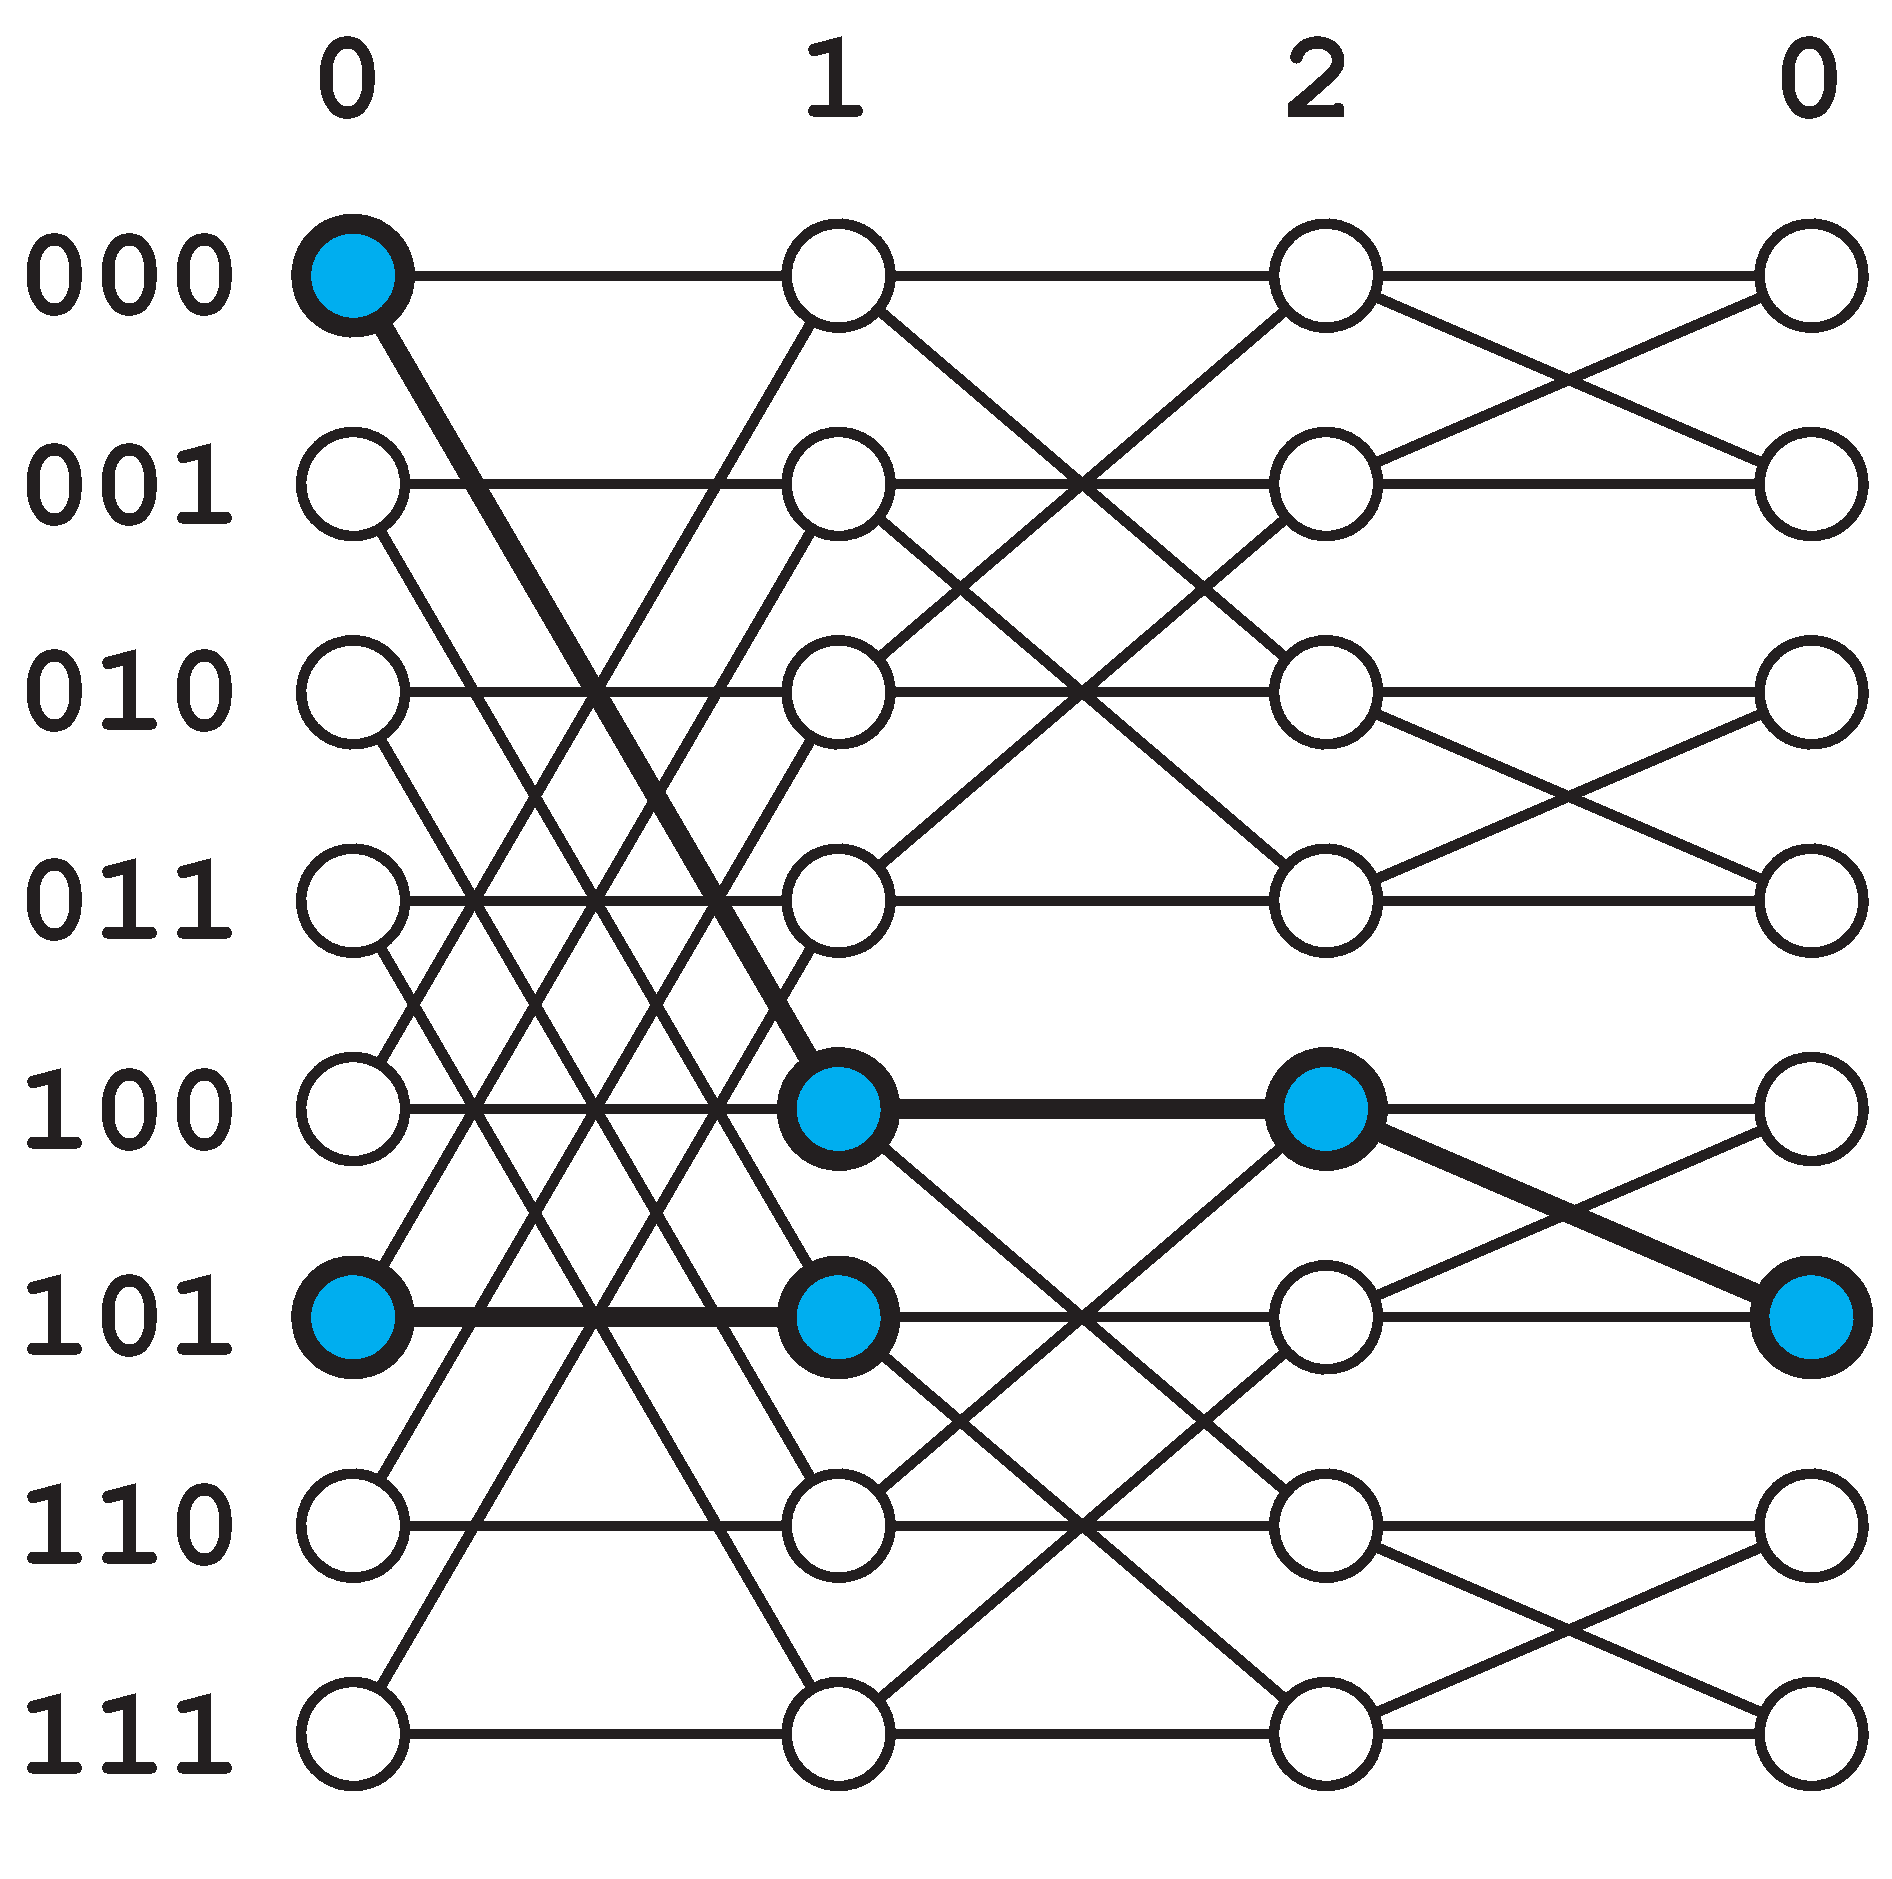
\includegraphics[width=2.66in]{fig-bf-route}
%\end{center}
%\caption{
%A 3-dimensional wraparound butterfly network.
%Note that the rightmost nodes are the same nodes as the leftmost,
%drawn twice for visual clarity.
%The highlighted nodes and edges show the path from node (0,000)
%to node (1,101).
%\label{fig:bf-route}
%}
%\end{figure}

%\begin{figure}[h]
%\begin{center}
%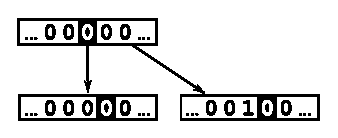
\includegraphics{fig-butterfly}
%\end{center}
%\caption{
%Schematic illustration of the two types of edges in a directed butterfly
%network.
%The node $(l,z)$ is shown as the bit string $z$ with a square around the
%$l$th bit.
%``Down'' edges increment $l$, leaving $z$ unchanged,
%while ``down-right'' edges increment $l$ and invert the $l$th bit of $z$.
%In the wrap-around variant, the nodes with maximum $l$ have down and down-right
%edges to the nodes with $l=0$.
%\label{fig:butterfly}
%}
%\end{figure}

The wrap-around butterfly network is known to have several of the properties
we desire for scalable, decentralized communication networks:
\begin{description}
\item[Vertex-transitivity:]
Because the wrap-around butterfly is vertex transitive,
it is maximally decentralized;
\item[Small-diameter:]
For any two nodes, the length of the shortest path between them is
$O(\log N)$, where N is the number of nodes in the network
(corresponding to low-latency in real-world terms);
\item[Sparsity:]
With a constant degree of 4, the wrap-around butterfly is extremely sparse,
and can scale indefinitely without node degree becoming a limitation;
\item [Redundancy:]
Multiple paths exist between any two nodes.
Specifically, we will prove below that the number of
$h$-internally vertex-disjoint paths between two
nodes increases exponentially with $h$.
\end{description}

The structure of the butterfly network lends itself to a well-known
(unipath) routing algorithm,
which we later extend to the multipath case.
The unipath algorithm first follows a down or down-right edge at every step,
increasing the level $l$ by 1 and cycling through the
indices of the place-within-level.
If the current node's place-within-level matches the destination node's at
index $l$,
a down edge is chosen and the place-within-level does not change.
Otherwise, a down-right edge is chosen and the $l$th component of the
place-within-level is flipped,
after which it matches the destination.
After $m$ iterations of this, all levels have been visited
and the place-within-level matches that of the destination.
Simply following down (or up) edges will then increment (decrement) the
level until the destination node is reached.

\subsection{Butterfly Rewiring}

Even when a butterfly topology cannot be implemented perfectly,
it can still increase the attack tolerance properties of a network.
Here, we simulate targeted attacks against a snapshot of the internet's
router network on January 2, 2000
\cite{leskovec_graphs_2005}, having 6493 nodes and 13914 edges.
At each step of the simulation, betweenness centrality is recalculated and the
most central node is removed.
We also simulate attack on several rewired networks.
The rewiring process alters the network structure to resemble a butterfly
topology, without adding any additional edges.
We 1. generate edges corresponding to a 9-dimensional butterfly network between
the 4608 highest-degree router nodes,
2. choose a fraction $f$ of those edges at random,
3. add those edges to the router network, and
4. remove an equal number of the original edges at random.

Our simulations show improved resistance to fragmentation and higher
effective redundancy when even a fraction of edges have been rewired to
match the butterfly topology.
While the original router network fragments when about 1\% of the nodes
have been removed (Fig. \ref{fig:diameter}),
this number increases to 2\%
with only 10\% of the butterfly edges present.
With 90\% of the butterfly edges present
the network remains unfragmented beyond the failure of the 8\% most
central nodes.

\begin{figure}
\begin{center}
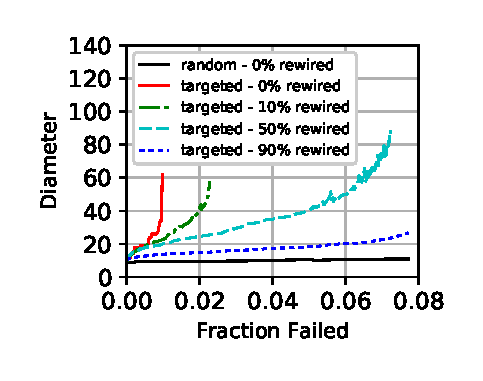
\includegraphics[width=2.5in]{fig-diameter}
\caption{
Simulation of targeted attacks against a snapshot of the internet's router
network with a fraction of the edges rewired into a partial butterfly configuration.
The original network fragments when the top 1\% of nodes are removed.
With only 10\% of the butterfly edges present,
this value doubles to 2\%.
}
\end{center}
\label{fig:diameter}
\end{figure}

%\begin{figure*}[h]
%\centerline{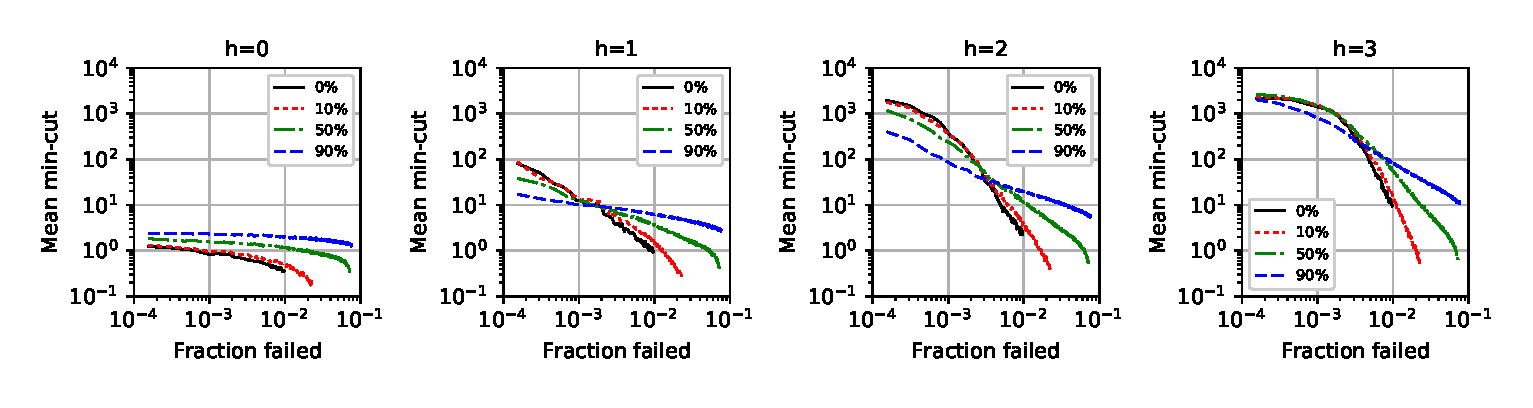
\includegraphics[width=6in]{fig-mincut}}
%\caption{
%Simulation of targeted attacks against a snapshot of the internet's router
%network with a fraction of the edges rewired into a partial butterfly configuration.
%The effective redundancy is shown for several values of trust transitivity $h$.
%For $h>0$, the original network has higher effective redundancy up to a crossover point,
%after which the rewired network performs better.
%}
%\label{fig:mincut}
%\end{figure*}

\section{Multipath Butterfly Routing}
\label{sec-bf-route}

We now present a routing algorithm to construct $2^h$
$h${\em-internally vertex-disjoint} paths
between two nodes in a butterfly network,
where $h$ is minimum distance from an endpoint to a compromised node.
Informally, Alice sends each message $h$ hops,
then to a distinct intermediate node,
then to a node $h$ hops from Bob, and finally to Bob.
The intermediate nodes are in a sense ``far'' from each other and ensure that
no two paths overlap.
Each path can be parameterized by a single integer $s$.

%\begin{table}[h]
%\caption{Butterfly Multipath Routing Variables\label{tab:routing}}
%\begin{center}
%\begin{tabular}{ll}
%Name & Variable \\\hline
%butterfly dimension & $m \in \mathbb{Z}_+$ \\
%node level & $l \in \mathbb{Z} : 0 \leq l < m$ \\
%node place within level & $z \in \mathbb{Z}_2^m$ \\
%trust radius & $h \in \mathbb{Z} : 1 \leq h \leq \lfloor m/2 \rfloor$ \\
%path index & $s \in \mathbb{Z}_2^h$ \\
%\end{tabular}
%\end{center}
%\end{table}

%\begin{figure}[h]
%\begin{center}
%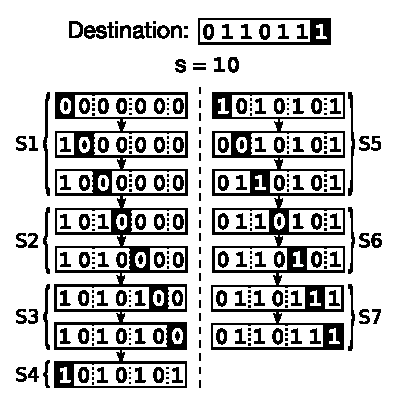
\includegraphics{fig-routing}
%\end{center}
%\caption{
%An example of one path as constructed by the proposed multipath
%routing algorithm.
%The path is shown for $s = 10_2$
%and $w = (6, 0110111_2)$.
%\label{fig:routing}
%}
%\end{figure}

\subsection{Algorithm Specification}

We now begin the formal specification of our multipath routing scheme for the
wrap-around butterfly network.
Utilizing vertex transitivity, we label the source node as
$(l^{(0)}, z^{(0)}) = (0, 0)$ and denote the destination node as $w = (l_w, z_w)$,
without loss of generality.

Let $s$ be an $h$-bit binary string with $s_i$ denoting the bit at index $i$.
There are $2^h$ such strings.
Let $v_s^{(t)} = (l^{(t)}, z^{(t)})$ be the node at position $t$
in the path parameterized by $s$.
For convenience,
we will omit the subscript $s$ when it is obvious from context.
We define three distinct partitions of $m$-bit binary strings.
Let $Q_{v^{(0)}}$ be the set of $m$-bit
strings in which the bits at
all indices $h \leq i < l_w - h$ match those of $z^{(0)}$,
and let $\overline{Q_{v^{(0)}}}$ be its complement.
Note that $Q_{v^{(0)}}$ is trivially all $m$-bit strings if $l_w < 2h$.
Let $R_s$ be the set of $m$-bit strings with the lowest $h$
bits all matching the bits of $s$,
and let $\overline{R_s}$ be its complement.
Let $S_s$ be the set of $m$-bit strings with the $h$ bits
preceding index $l_w$ all matching the bits of $\tilde{s}$,
where $\tilde{s}$ is a cyclic permutation of $s$:
\beq
\tilde{s}_i &=& s_{(i + l_w) \text{ mod } h},
\eeq
and let $\overline{S_s}$ be its complement.
We will make use of the fact that:
\beq
s \neq s^\prime &\implies&
S_s \cap S_{s^\prime} = R_s \cap R_{s^\prime} = \emptyset.
\eeq

Routes are constructed in 7 stages.
The network topology dictates that $l^{(t+1)} = l^{(t)} + 1$ (mod $m$),
so we let $l = t$ (mod $m$).
and that $z^{(t+1)}$ is equal to $z^{(t)}$ with or without the bit in index
$l^{(t)}$ inverted, depending on whether the down or down-right edge was
taken at step $t$.
\begin{description}
\item[Stage 1: ($0 \leq t < h$)]{
Down or down-right edges
are chosen such that the $t$th bit of $z^{(t+1)}$ is equal to the $t$th bit
of $s$.
Throughout Stage 1, all nodes are within the sender's trusted neighborhood.
Throughout Stage 1, $z^{(t)} \in Q_{v^{(0)}}$.
At the end of Stage 1, $z^{(h)} \in S_s$, and $z^{(t)}$ will remain so until the level cycles to $0$ at $t = m$.
}
\item[Stage 2: ($h \leq t < l_w - h$)]{
Edges are chosen to make the $t$th bit of
$z^{(t+1)}$ the inverse of the $t$th bit of $z^{(0)}$.
Note that this stage does not occur when $l_w < 2h$.
If this stage occurs, then $z^{(t)} \in \overline{Q_{v^{(0)}}}$ until these
levels are reached again in stage 6.
}
\item[Stage 3: ($l_w - h \leq t < l_w$)]{
The bits of $z^{(t)}$ are chosen to match $\tilde{s}$,
such that after the stage is complete, $z^{(t)} \in R_s$.
}
\item[Stage 4: ($l_w \leq t < m$)]{
Paths are chosen such that the $t$th bit of $z^{(t+1)}$ matches that of the
destination node $z_w$.
This stage will not occur if $l_w > m - h$.
}
\item[Stage 5: ($m \leq t < m + h$)]{
There are two cases.
If $2h < l_w < m - h$,
then there is no overlap between the indices defining $R_s$ and $S_s$.
In this case, the first $h$ bits of $z^{(t)}$ are set to
match $z_w$.
Otherwise there is some overlap between the indices defining $R_s$ and
$S_s$.
In this case, the each of the first $h$ bits of $z^{(t)}$ is either kept the
same if $l_w - h \leq l < l_w$, or set to the corresponding bit of $z_w$
otherwise.
In this stage and after, $z^{(t)}$ is no longer guaranteed to be in $R_s$.
However, $z^{(t)}$ remains in $S_s$ during and after this stage.
}
\item[Stage 6: ($m + h \leq t < m + l_w - h$)]{
In this stage, edges are chosen to set the bits of $z^{(t)}$ to their
corresponding value in $z_w$.
$z^{(t)} \in \overline{Q_{v^{(0)}}}$ throughout this stage,
but not afterwards.
}
\item[Stage 7: ($m + l_w - h \leq t < m + l_w$)] {
The $h$ bits of $z^{(t)}$
preceding index $l_w$ are set to match $z_w$.
All nodes in this stage are within $h$ hops of $w$ and thus in its trusted
neighborhood.
After this stage, $v^{(m + l_w)} = w$ and routing is complete.
}
\end{description}

\subsection{Proof of Path Independence}

\begin{theorem}
Given an $m$-bit wrap-around butterfly network ($m > 1$),
and an integer $h$ ($1 \leq h \leq \left\lfloor \frac{m}{2} \right\rfloor$),
for all node pairs $(v, w)$ such that $d(v,w) \geq 2h$,
there exist at least $2^h$ $h$-internally vertex disjoint
paths $v_s$ ($0 \le s < 2^h$) from
$v$ to $w$ such that
$s \neq s^\prime \implies v_s \cap v_{s^\prime} \subset T_h(u) \cup T_h(v)$.
\end{theorem}
\begin{proof}
Nodes from two paths can only coincide if their levels are the same.
Nodes which share a level must either be in the same stage, or 4 stages
apart.
Let ($a$,$a^\prime$) denote a pair of sub-paths corresponding to stage $a$ of
one path and stage $a^\prime$ of another.
Excluding paths that intersect in their trusted neighborhoods, (1,1) and (7,7),
we have reduced the list of possible intersections to the following cases:
(2,2), (3,3), (4,4), (5,5), (6,6), (1,5), (2,6), and (3,7).
Nodes in stages 2--4 belong to $R_s$ so cannot overlap with any stage 2--4
nodes from another path, eliminating (2,2), (3,3), and (4,4).
Similarly, nodes in stages 4--6 belong to a unique $S_s$,
eliminating (5,5) and (6,6).
Nodes in stage 1 belong to $Q_{v^{(0)}}$ while those in stage 5 belong in
its complement, eliminating (1,5).
Similarly, for all $l$ in stage 2, $z^{(l)}$ is equal to $z^{(0)}$,
while in stage 6, $z^{(l)}$ is the inverse, eliminating (2,6)
This leaves only (3,7), a collision which can occur only for only one path
(with $s$ matching the first $h$ bits of $z_w$), and which enters the trusted
neighborhood in stage 3.
For this single path, we can proceed directly from stage 2 to stage 7,
eliminating the last possible collision.
\end{proof}

\section{Discussion}
\label{sec-discussion}

In its current form, our work has several limitations.
Most obviously, it requires control over the network structure.
However, we have shown that even partial control over network structure can
improve attack tolerance properties.
There is also the question of how to construct such a network without a central
authority.
We conjecture that smaller independently-formed networks could be
merged into a single larger network without central coordination.
When nodes are tied to geographic locations,
the butterfly topology would require connections between very distant locations.
Such connections are extremely expensive to construct and maintain,
although they do exist in the form of internet backbones.
An alternative solution might involve satellite links,
which connect distant geographic points much more easily.
While turning our network theoretical results into practical applications
will require considerable additional work, we believe that work is inevitably
necessary in order to create attack-tolerant networks.

\section{Conclusion}
\label{sec-conclusion}

Coercion-resistant, topological approaches to attack tolerance are needed to
address the current vulnerability of communications infrastructure to
censorship and surveillance.
We have presented a novel concurrent multipath routing (CMR)
algorithm for the butterfly network,
as well as a structured multipath fault tolerance (SMFT) scheme,
which can be combined to create a coercion-resistant,
attack-tolerant point-to-point communication architecture.
Even when network structure cannot be perfectly controlled,
we have shown that partially rewiring a snapshot of the internet's router network
can greatly increase its attack-tolerance properties.
We believe that this work provides a foundation for the
development of topology-based 
architectures to guard against adversarial attacks,
including censorship and surveillance.

\section{Acknowledgments}

Anonymized for blind review.
%The authors would like to thank Tony Garnock-Jones, A. Frederick Dudley, and
%Nathaniel Bezanson for helpful conversations.
%This research was partly supported by the National Science Foundation under
%Grant No. IIS-1617820.

{\footnotesize \bibliographystyle{acm}
\bibliography{references}}


%\theendnotes

\end{document}







